\documentclass{standalone}
\usepackage{tikz}

\begin{document}

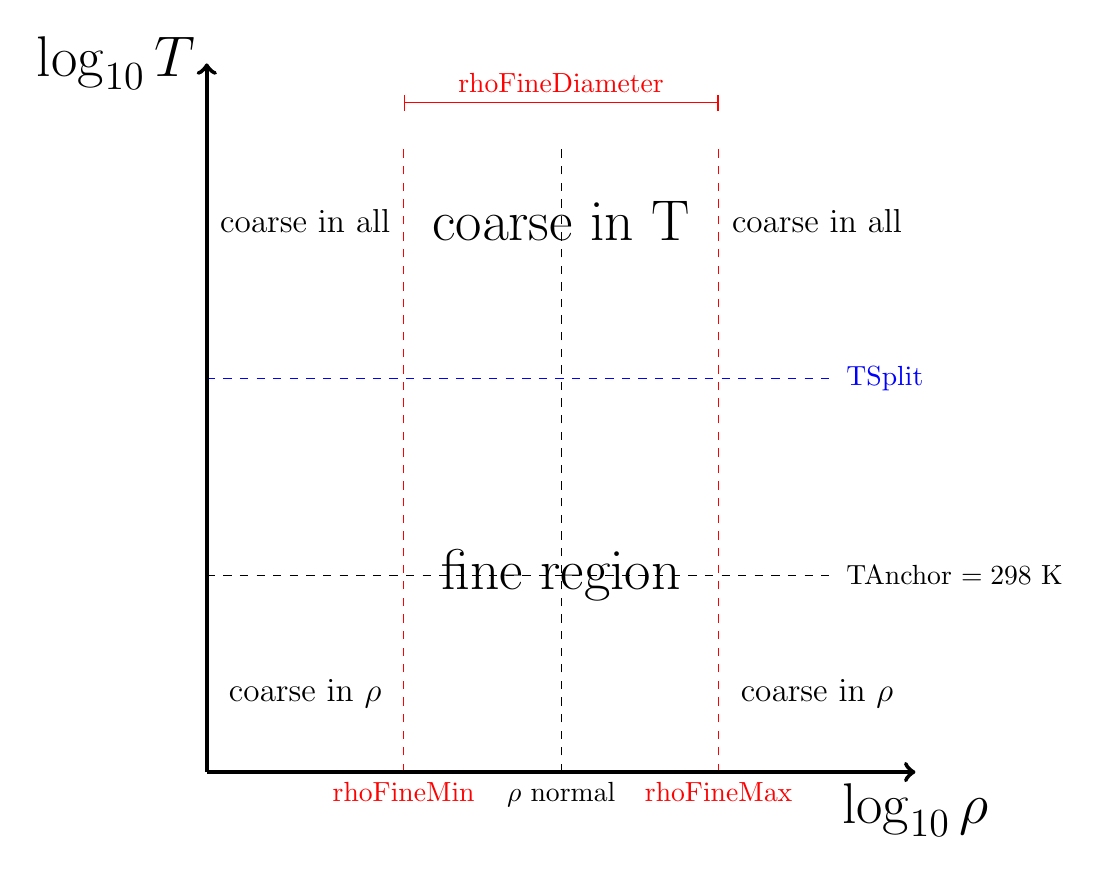
\begin{tikzpicture}
  \draw[dashed] (4.5, 0) -- ++(0,8);
  \draw (4.5, 0) node[below] {$\rho$ normal};
  \draw[red, dashed] (2.5, 0) node[below] {rhoFineMin} -- ++(0,8);
  \draw[red, dashed] (6.5, 0) node[below] {rhoFineMax} -- ++(0,8);
  \draw[red, |-|] (2.5,8.5) -- (6.5,8.5);
  \draw[red] (4.5, 8.5) node[above] {rhoFineDiameter};

  \draw[blue, dashed] (0, 5) -- ++(8, 0) node[right] {TSplit};
  \draw[dashed] (0, 2.5) -- ++(8, 0) node[right] {TAnchor $=298$ K};

  % Draw axes
  \draw[ultra thick,->] (0,0) -- (9,0) node[below] {\huge $\log_{10}\rho$};
  \draw[ultra thick,->] (0,0) -- (0,9) node[left] {\huge $\log_{10}T$};

  \draw (4.5, 2.5) node {\huge fine region};
  \draw (4.5, 7) node {\huge coarse in T};

  \draw (1.25, 1) node {\large coarse in $\rho$};
  \draw (7.75, 1) node {\large coarse in $\rho$};

  \draw (1.25, 7) node {\large coarse in all};
  \draw (7.75, 7) node {\large coarse in all};
\end{tikzpicture}

\end{document}